\documentclass{beamer}
\usetheme{Boadilla}

\usepackage{subcaption}
\usepackage{graphicx}

\title{Présentation phase 2 \textbf{infof209}}
\author{groupe 5 infof209}
\date{vendredi 21 mars 2025}

\begin{document}

\begin{frame}
\titlepage
\end{frame}

\begin{frame}[shrink=20]
\frametitle{Sommaire}
	\tableofcontents
\end{frame}

\section{Jeu}

\subsection{Implémentation des bases du jeu}
\begin{frame}
\frametitle{Implémentation des bases du jeu}

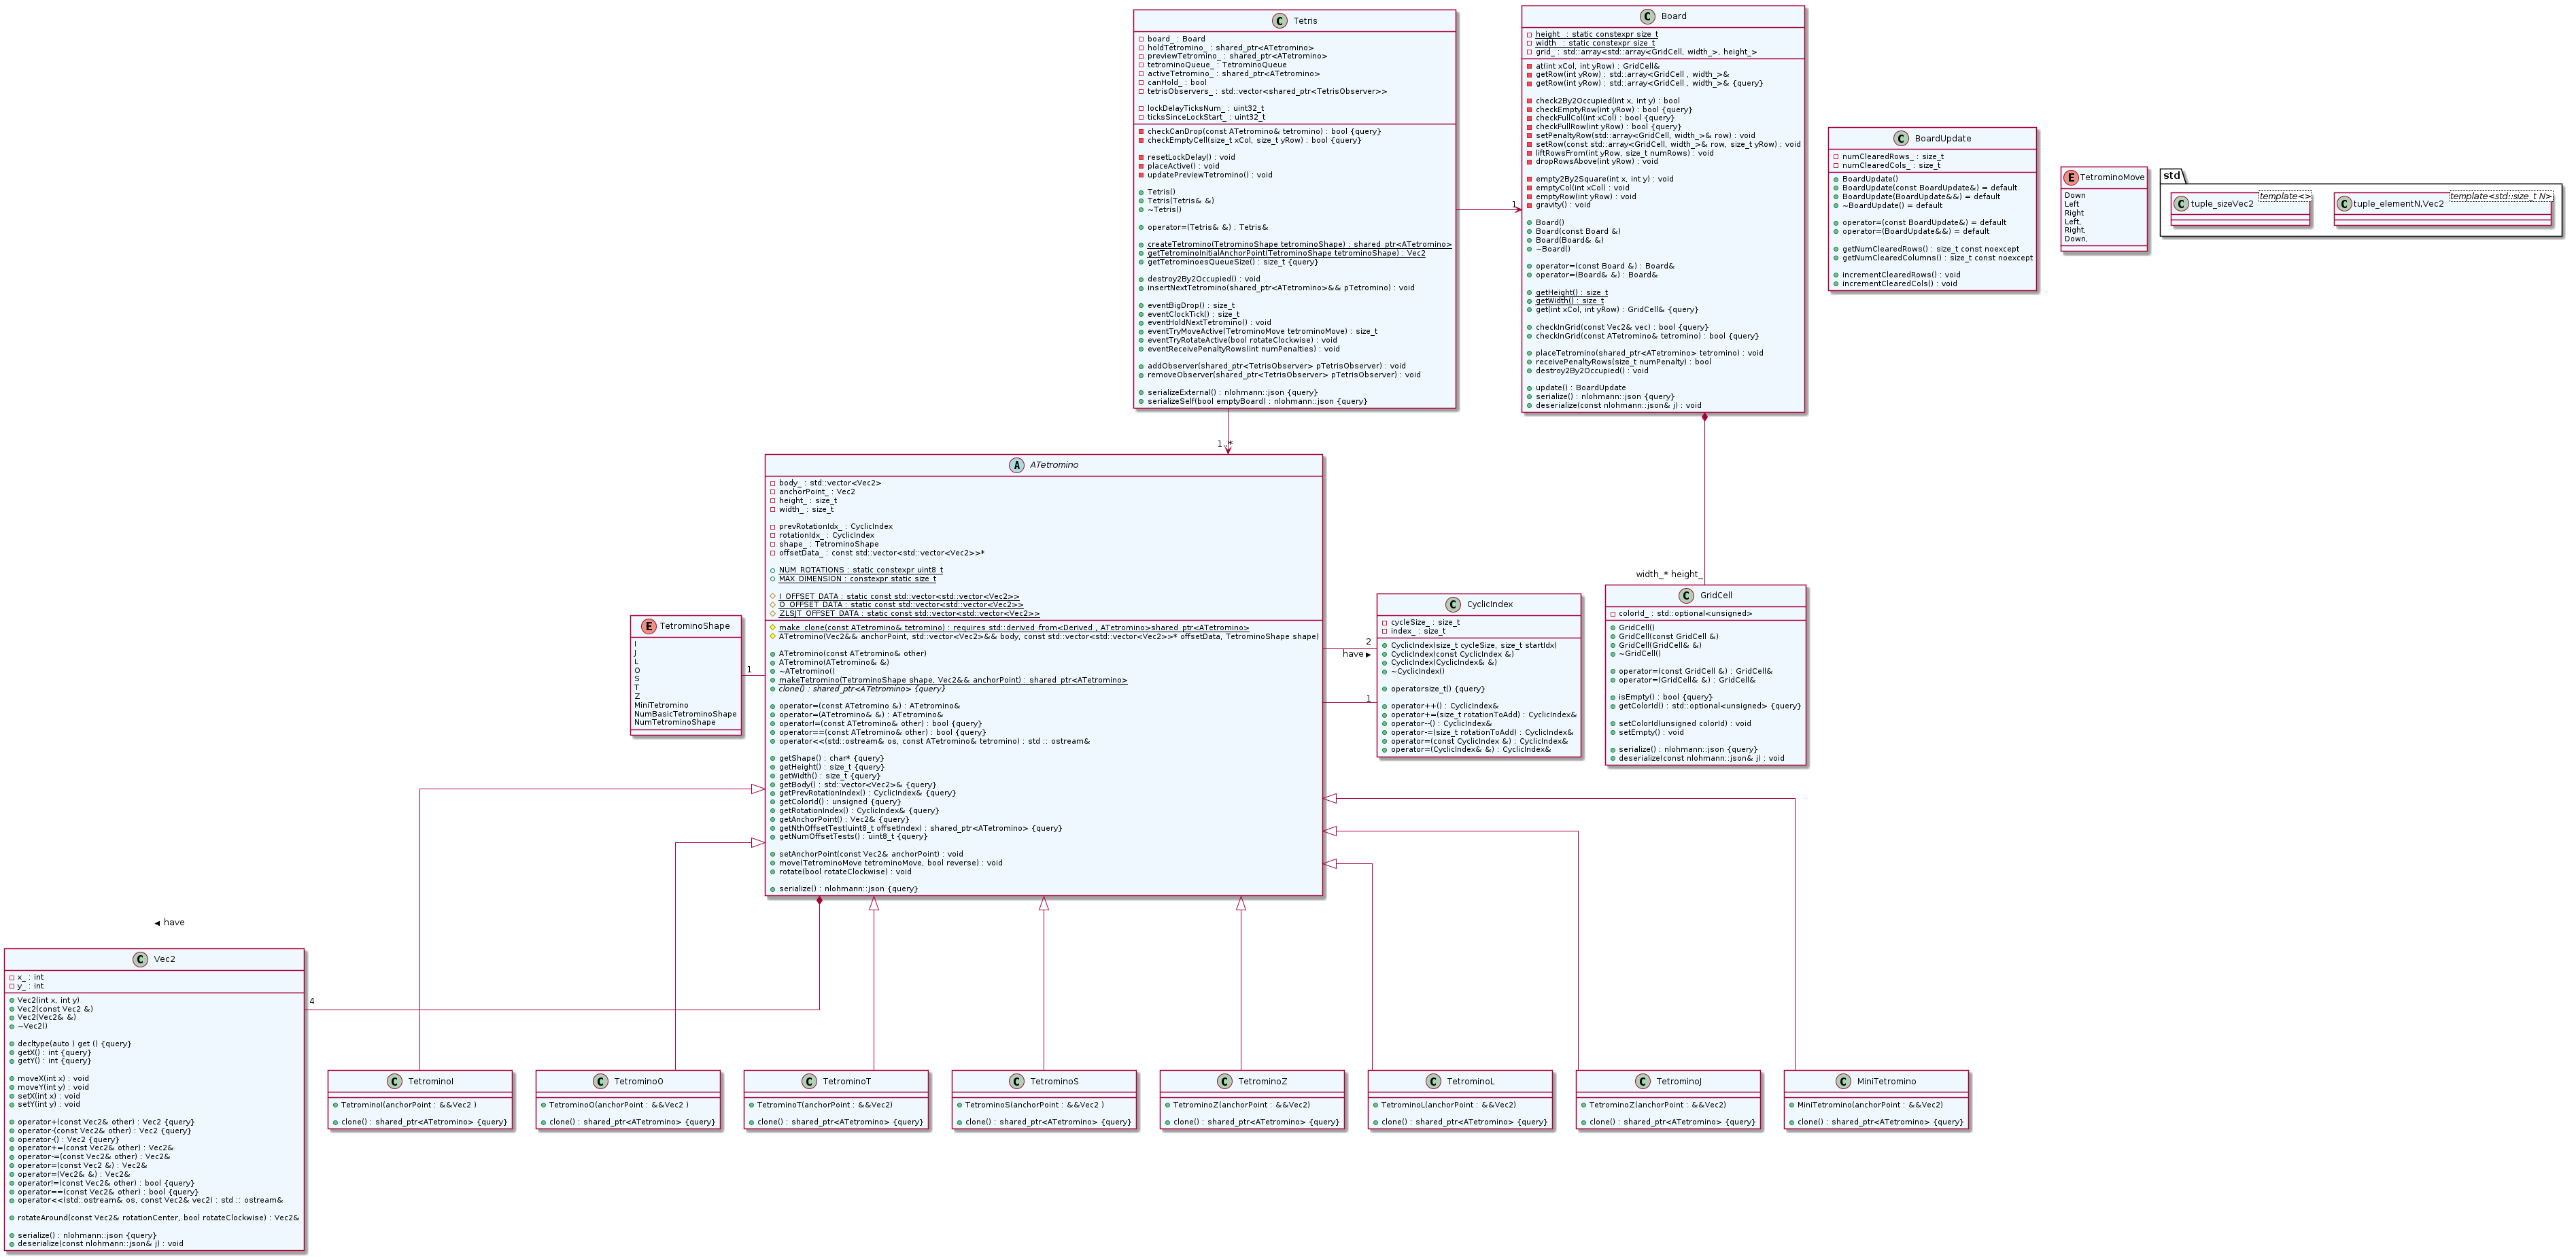
\includegraphics[width=1\textwidth]{../../res/uml/class/GameClass.png}

\end{frame}


\subsection{Implémentation des effects}
\begin{frame}
\frametitle{Implémentation des effects}

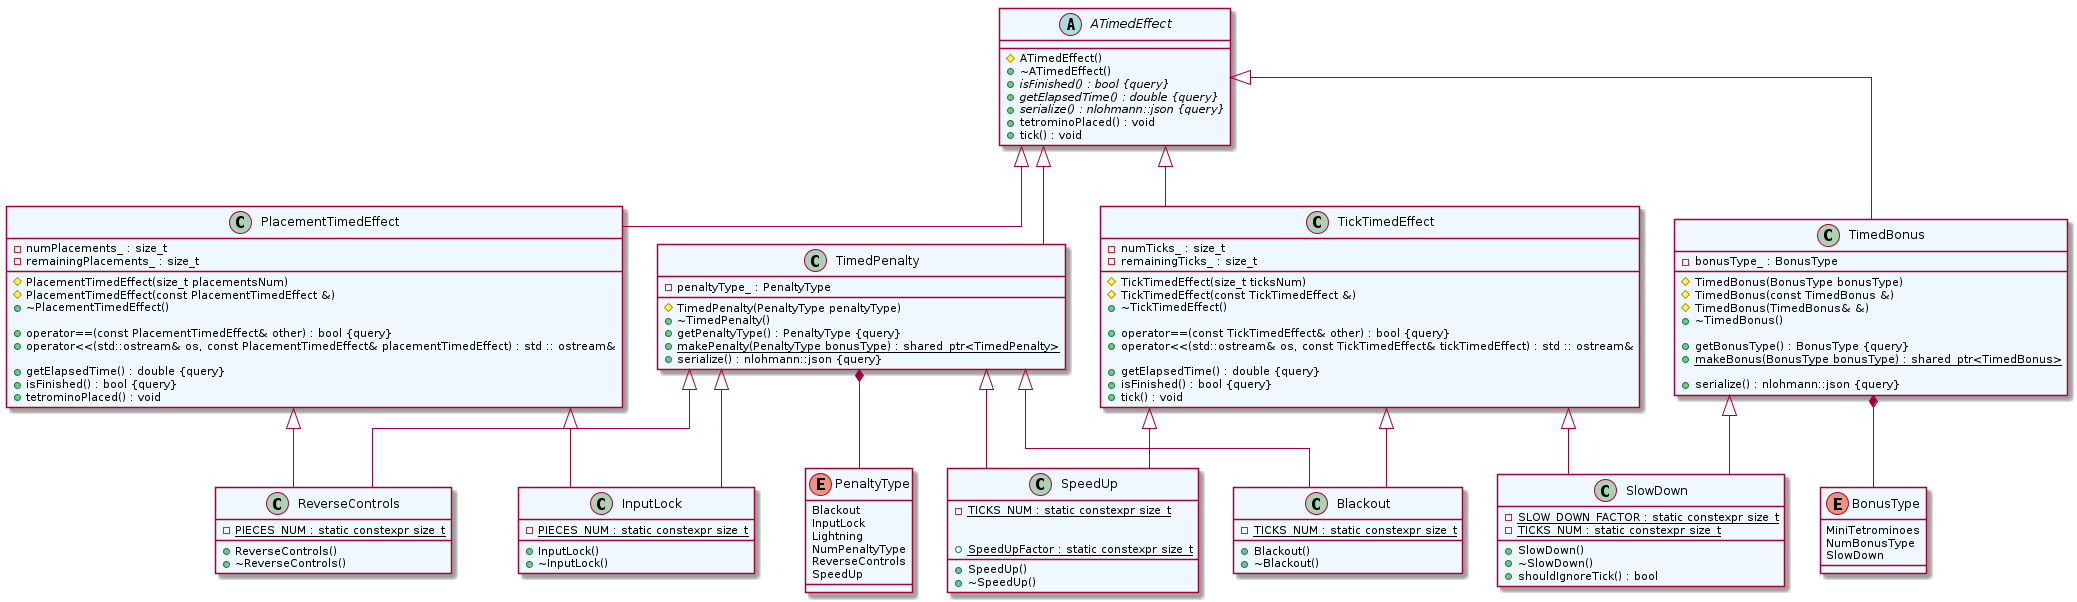
\includegraphics[width=1\textwidth]{../../res/uml/class/EffectClass.png}	
\end{frame}


\subsection{GameEngine}
\begin{frame}{GameEngine}

\begin{figure}

\centering
\hfill
\begin{subfigure}{0.3\textwidth}
    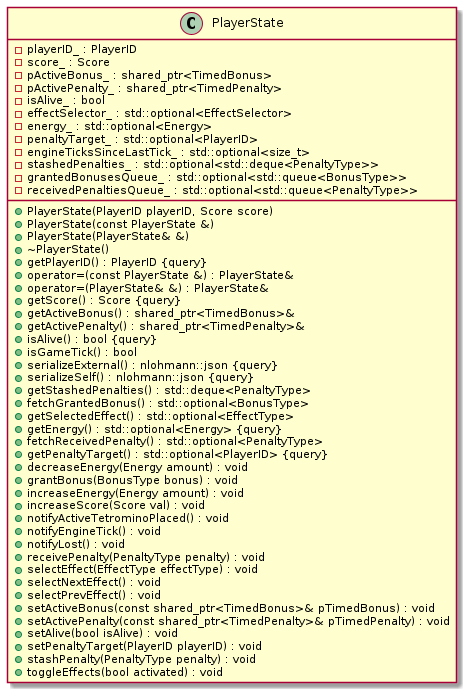
\includegraphics[width=\textwidth]{../../res/uml/class/PlayerStateClass.png}
    \caption{Diagramme de PlayerState}
    \label{fig:second}
\end{subfigure}
\hfill
\begin{subfigure}{0.2\textwidth}
    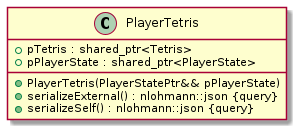
\includegraphics[width=\textwidth]{../../res/uml/class/PlayerTetrisClass.png}
    \caption{diagramme de PlayerTetris}
    \label{fig:third}
\end{subfigure}
\hfill
\begin{subfigure}{0.4\textwidth}
    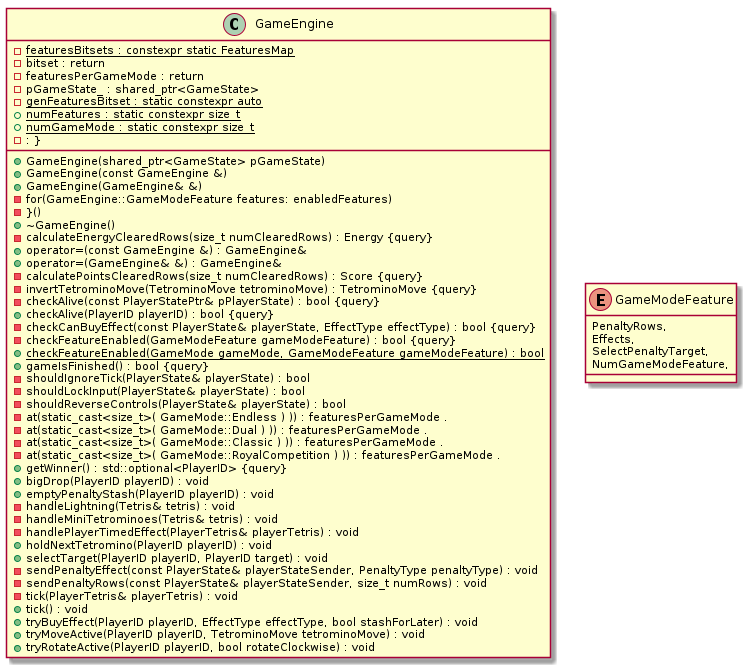
\includegraphics[width=\textwidth]{../../res/uml/class/GameEngineClass.png}
    \caption{Diagramme de GameEngine}
    \label{fig:first}
\end{subfigure}

\end{figure}

\end{frame}

\subsection{Implémentation générale}
\begin{frame}
\frametitle{Implémentation Générale du Jeu}

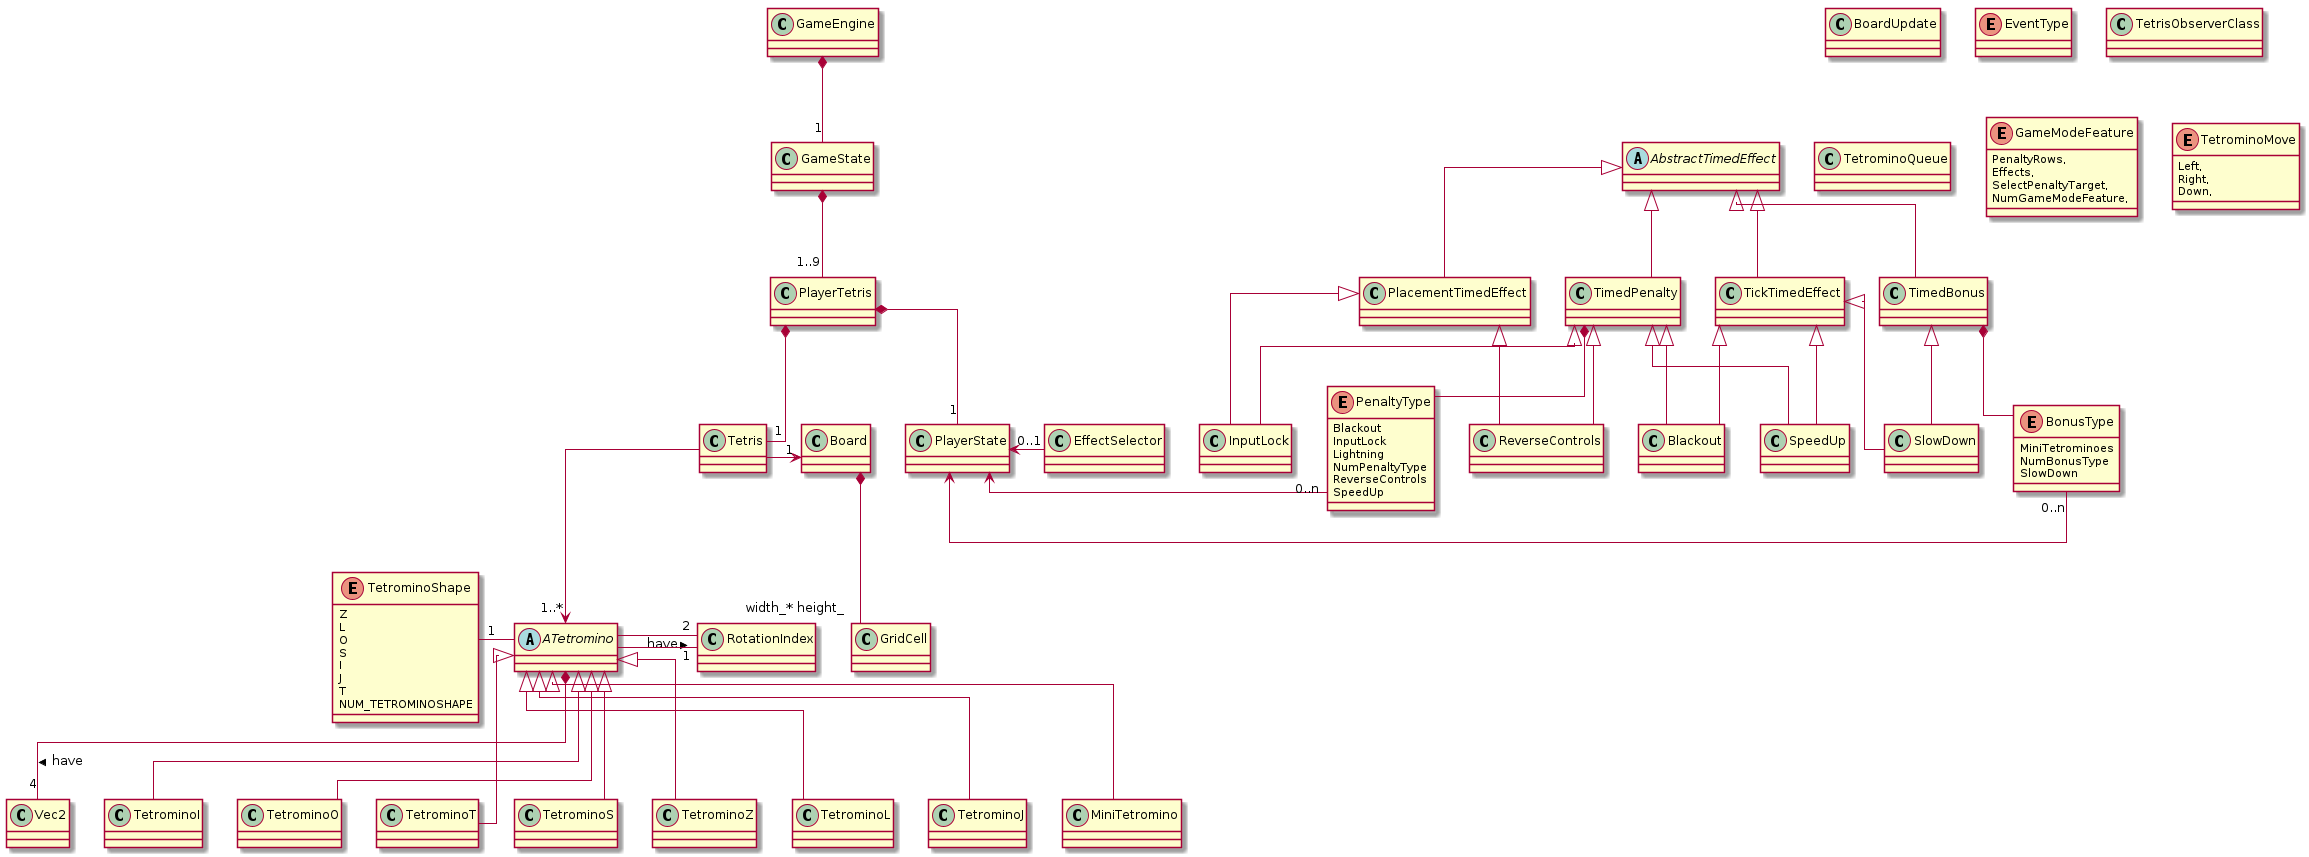
\includegraphics[width=1\textwidth]{../../res/uml/class/GameStructureClass.png}
\end{frame}

\section{Serveur}

\subsection{Choix des librairies et languages utilisées}
\begin{frame}
\frametitle{Choix des librairies et languages utilisées}

\begin{enumerate}
	\item Choix de SQLite
		\begin{itemize}
			\item compact
		\end{itemize}
	
	\item Choix de nlhomman/json
		\begin{itemize}
			\item json
		\end{itemize}
		
	\item Choix de boost/asio
		\begin{itemize}
			\item asynchrone
			\item io context = queue d'events - permet de gérer ticks  et client requests
		\end{itemize}
		
\end{enumerate}
\end{frame}

\subsection{Base de données}

\subsubsection{Structure de la base de données}
\begin{frame}
\frametitle{Structure de la base de données}

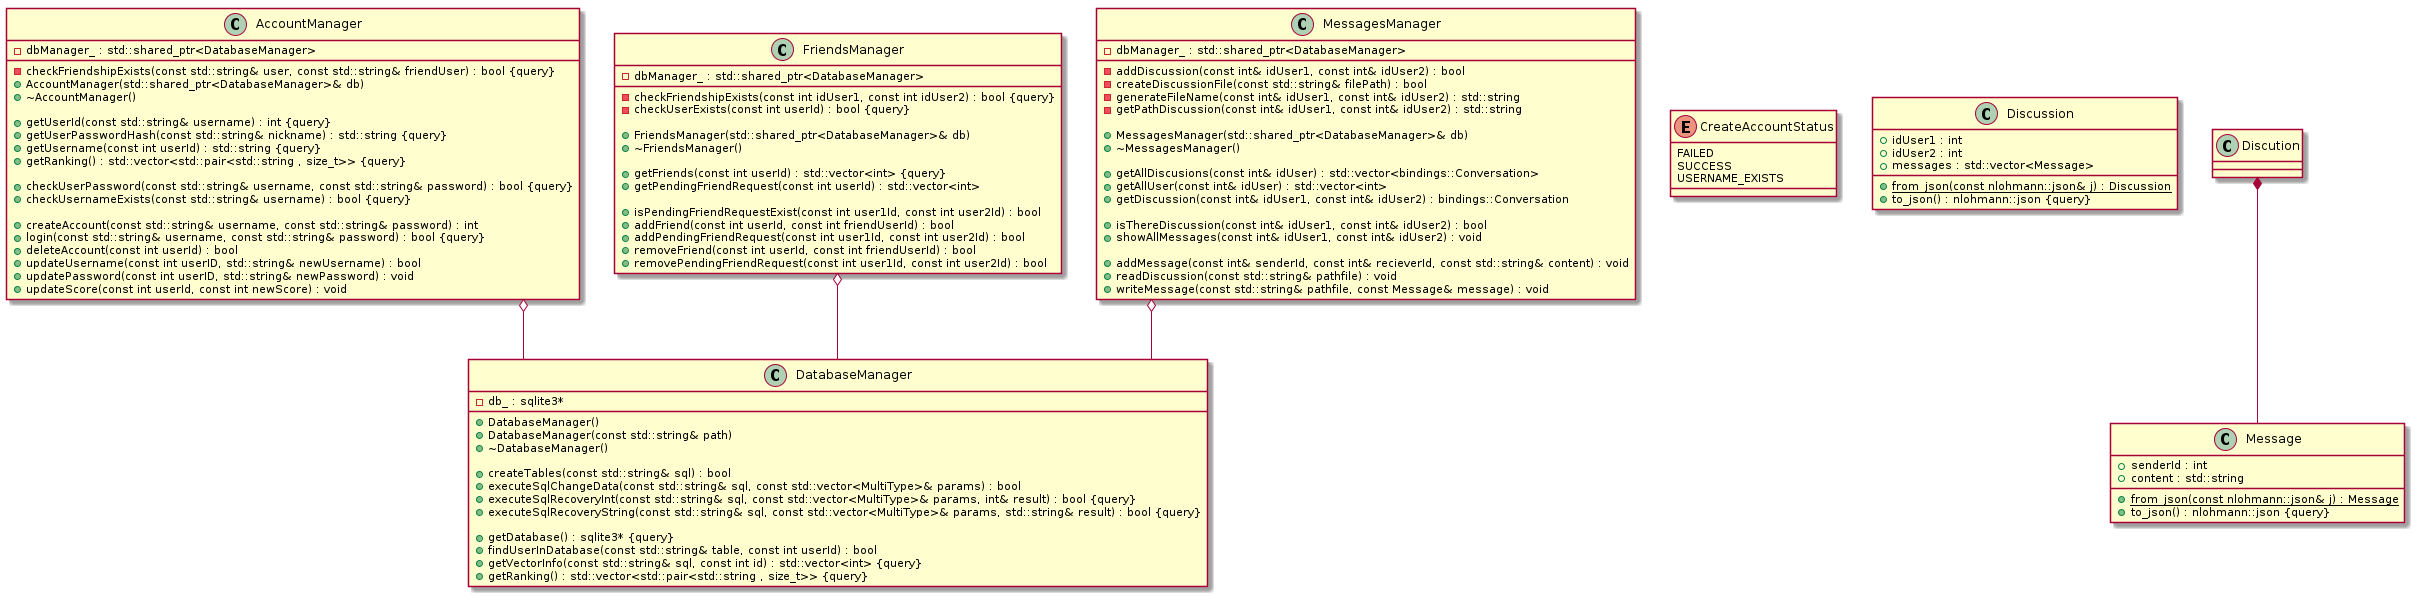
\includegraphics[width=1\textwidth]{../../res/uml/class/DatabaseClass.png}
\end{frame}

\subsection{Définition des bindings}
\begin{frame}
\frametitle{Définition des bindings}

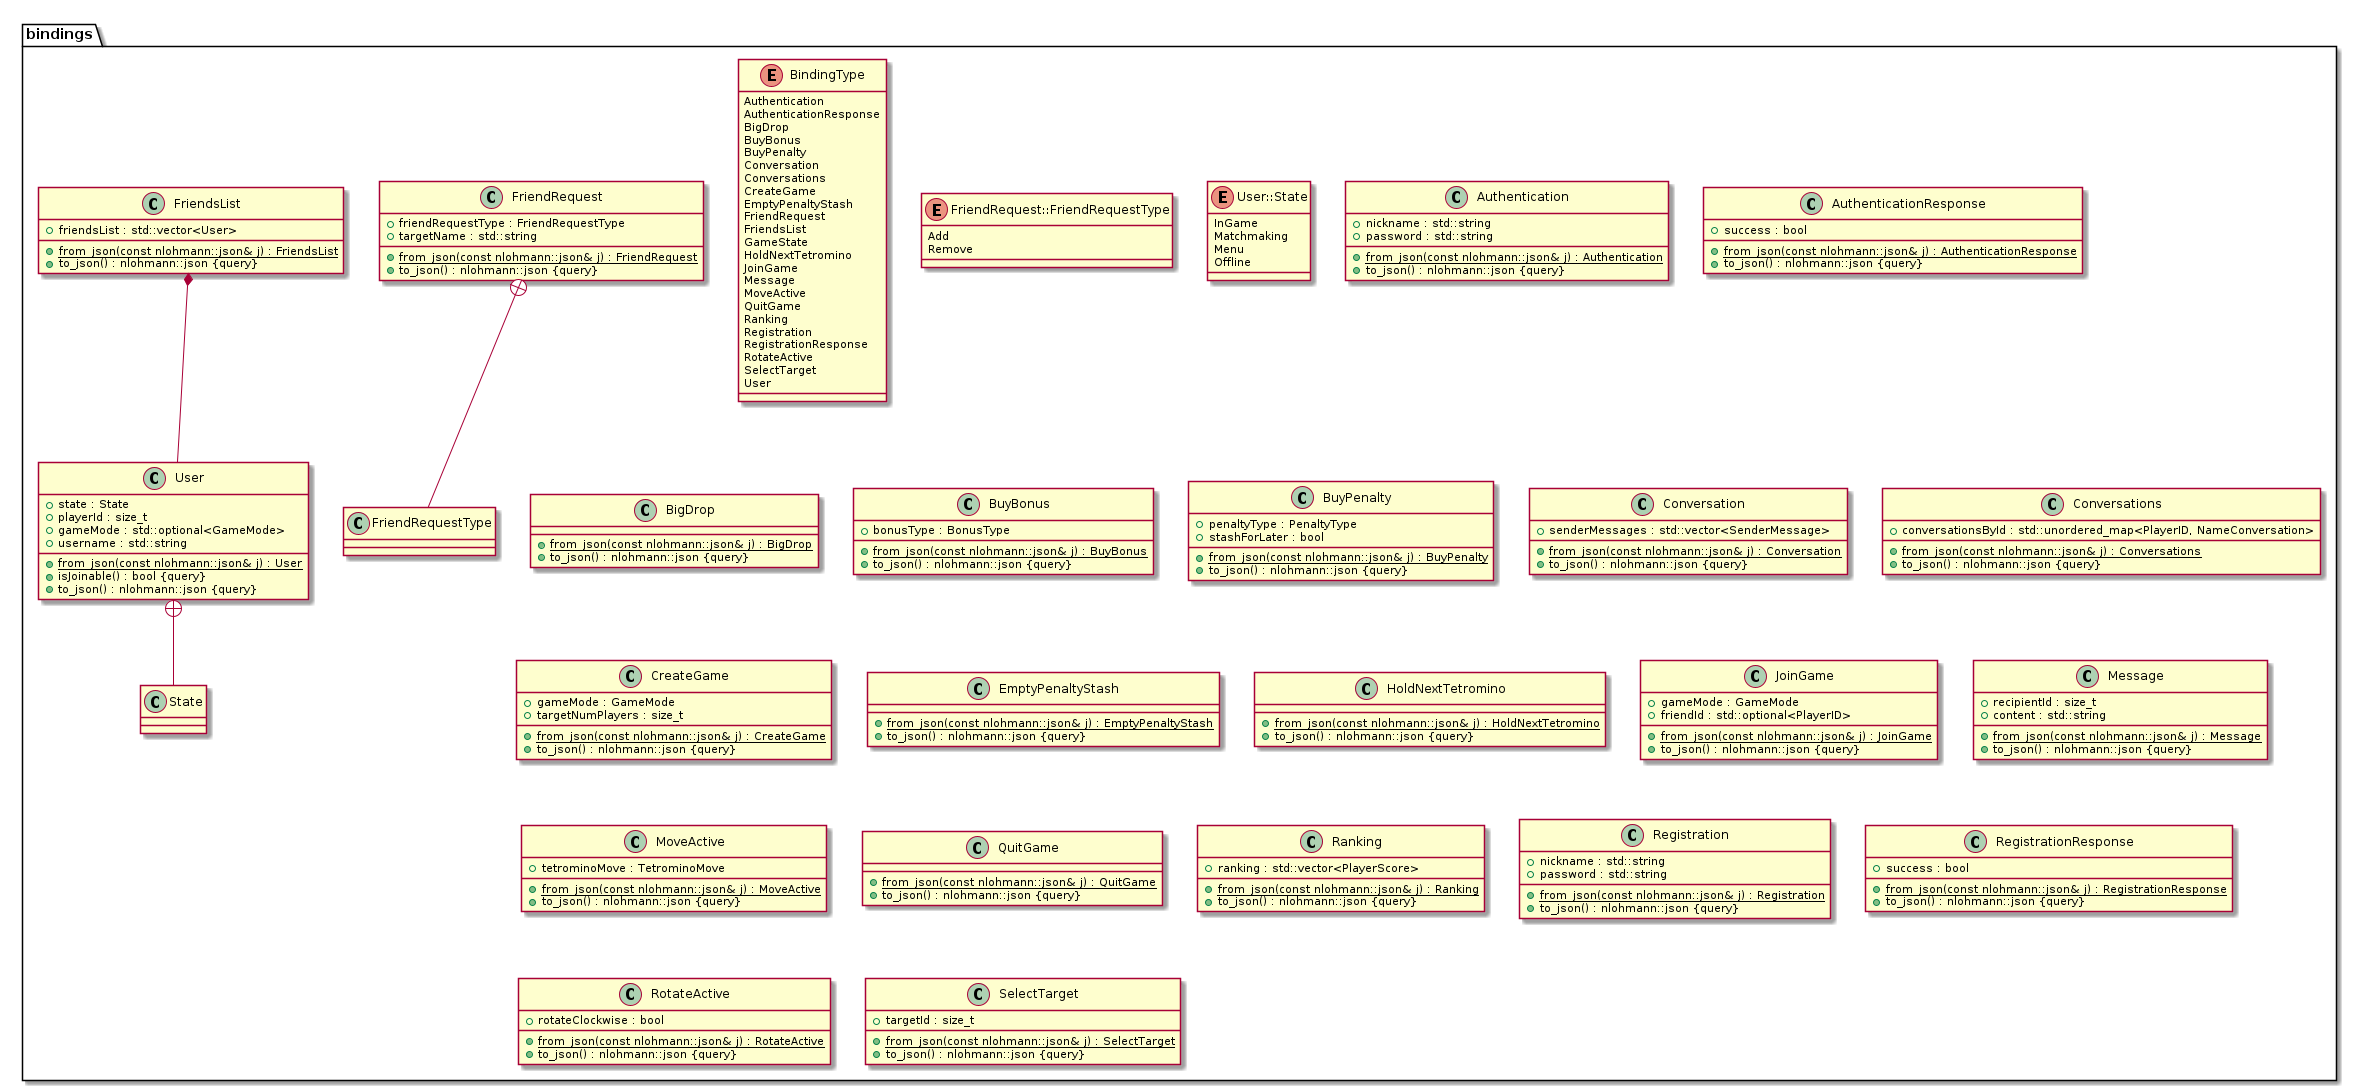
\includegraphics[width=1\textwidth]{../../res/uml/class/BindingClass.png}
\end{frame}


\subsection{Structure de GameServer}
\begin{frame}
\frametitle{Structure de GameServer}

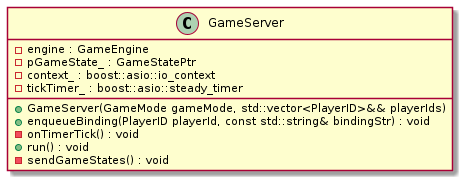
\includegraphics[width=1\textwidth]{../../res/uml/class/GameServerClass.png}
\end{frame}


\subsection{Structure de Network}


\subsubsection{Network}
\begin{frame}
\frametitle{Structure de Network}

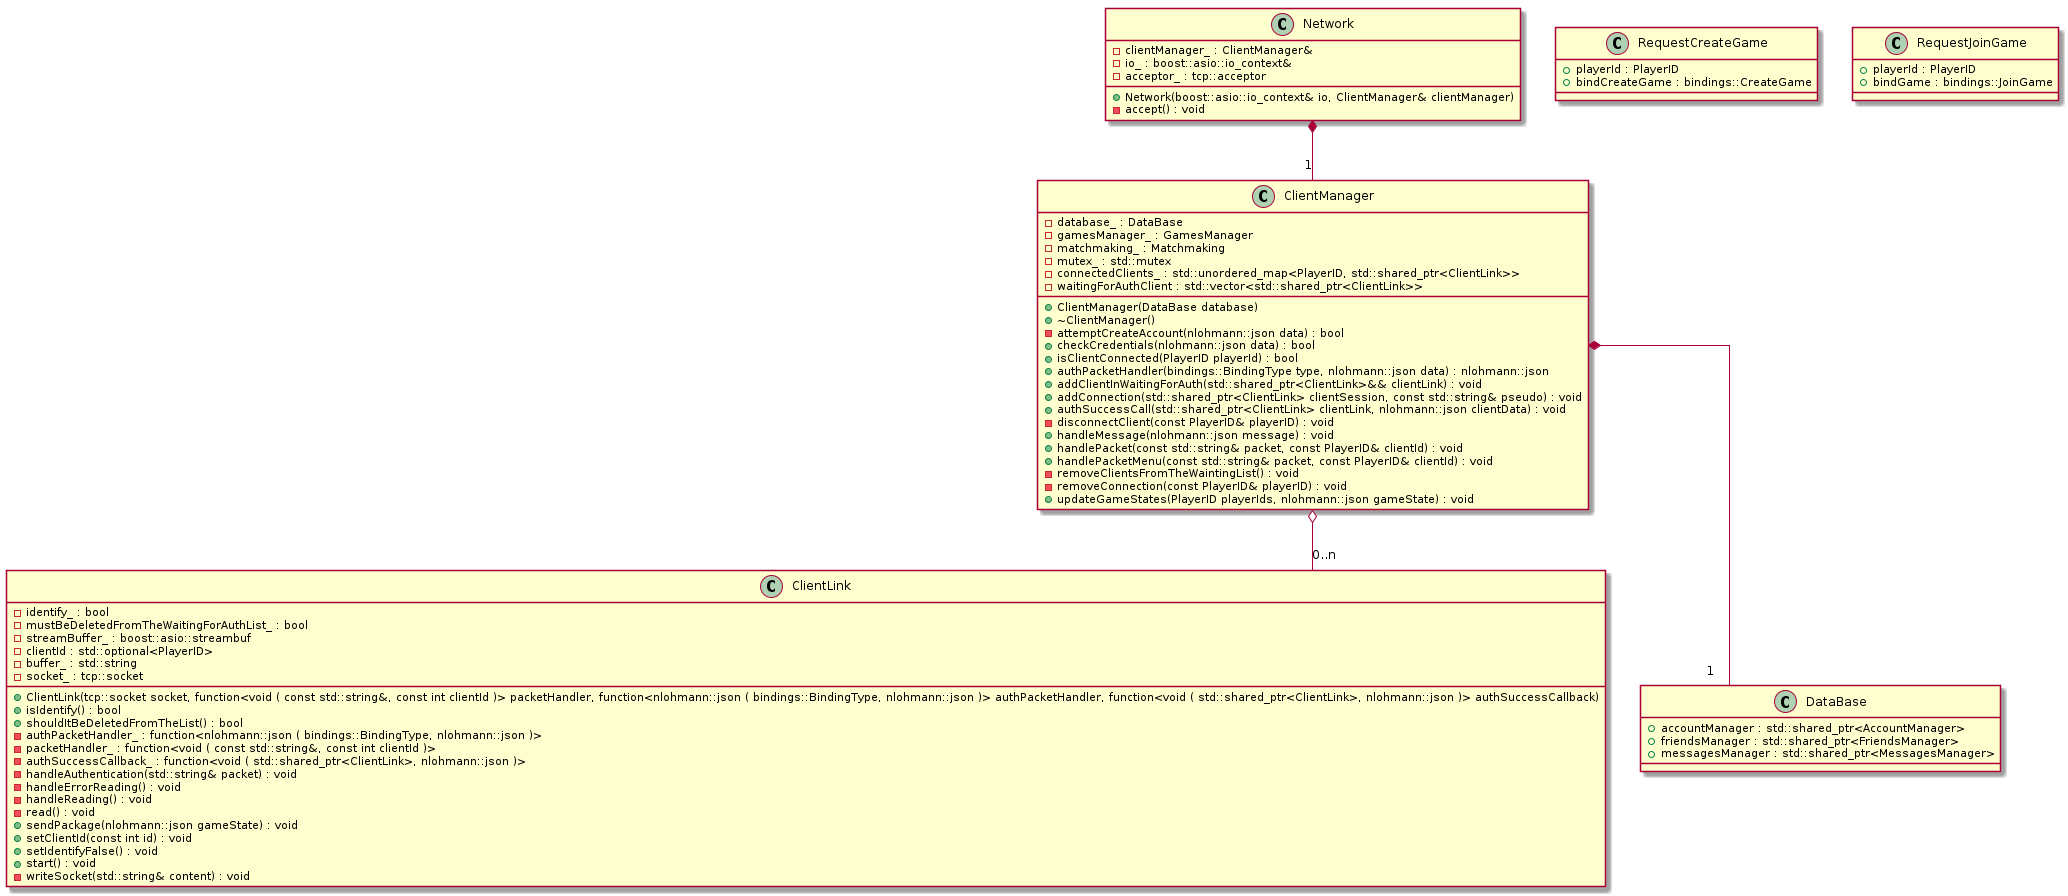
\includegraphics[width=1\textwidth]{../../res/uml/class/NetworkClass.png}
\end{frame}

\subsubsection{MatchMaking}
\begin{frame}
\frametitle{Structure de MatchMaking}

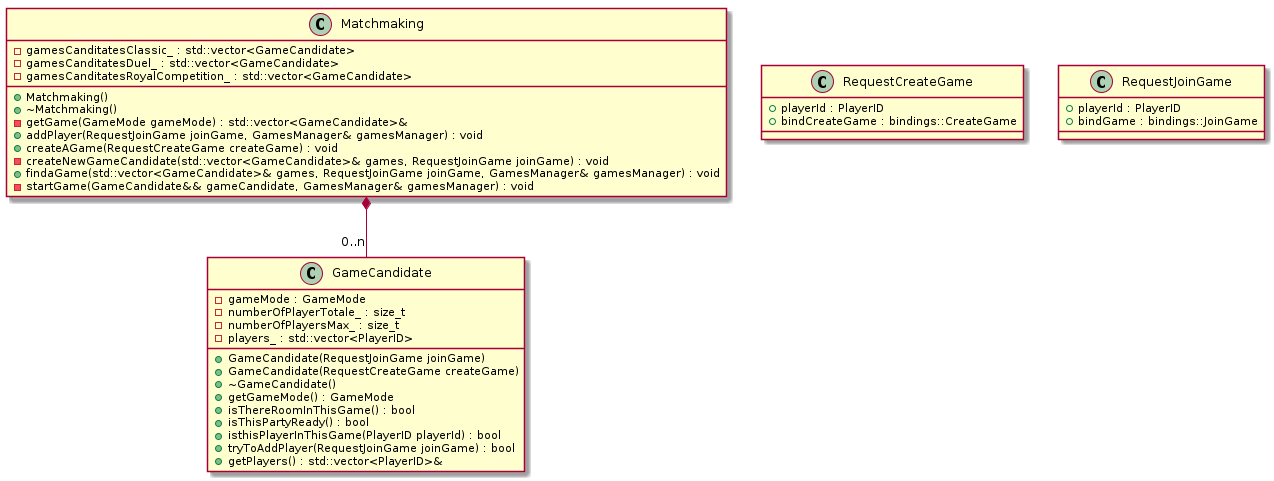
\includegraphics[width=1\textwidth]{../../res/uml/class/MatchMakingClass.png}
\end{frame}

\subsubsection{Implémentation générale}
\begin{frame}
\frametitle{Implémentation générale du Serveur}

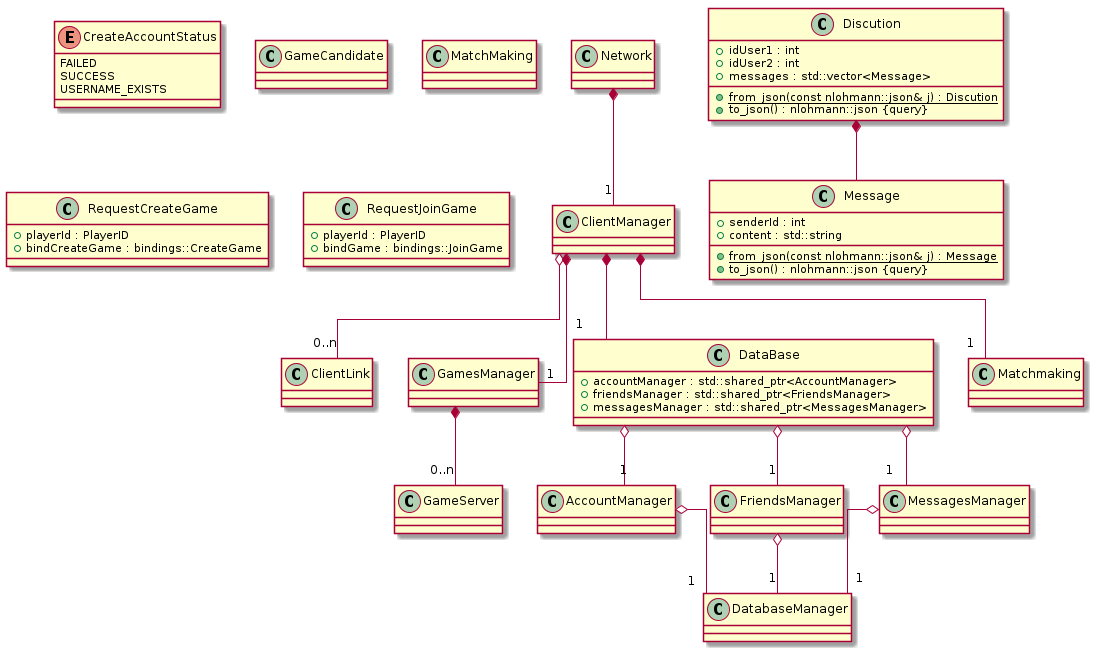
\includegraphics[width=1\textwidth]{../../res/uml/class/ServerStructureClass.png}
\end{frame}

\subsection{Fonctionnement}

\subsubsection{Game}
\begin{frame}
\frametitle{Fonctionnement d'une partie de jeu côté serveur}

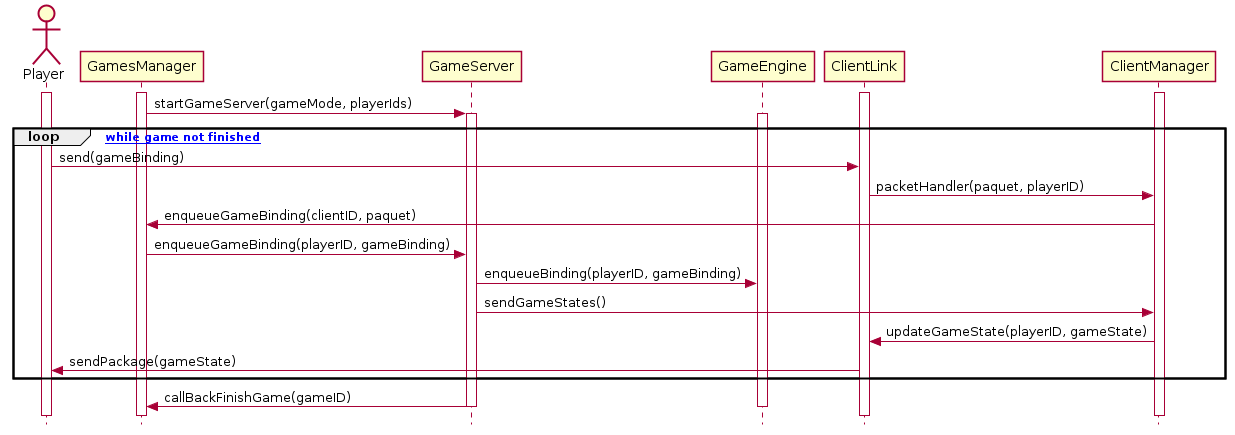
\includegraphics[width=1\textwidth]{../../res/uml/sequence/GameServerSequence.png}
\end{frame}

\subsubsection{Matchmaking}
\begin{frame}
\frametitle{Fonctionnement du Matchmaking côté serveur}

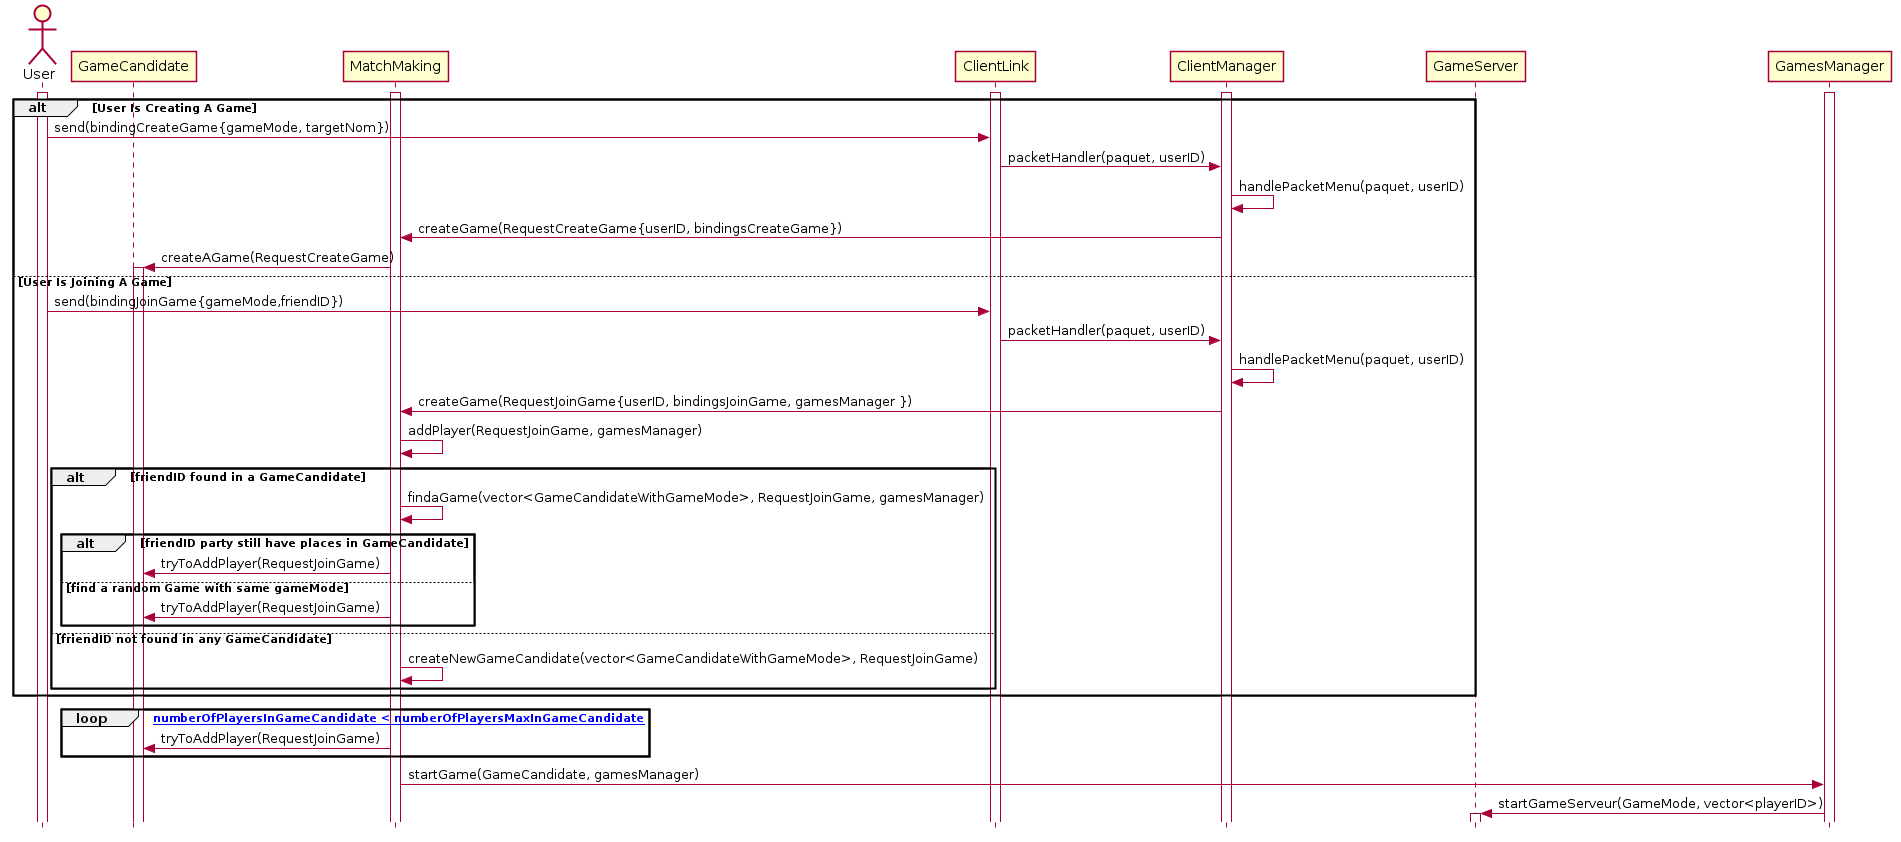
\includegraphics[width=1\textwidth]{../../res/uml/sequence/MatchMakingServerSequence.png}
\end{frame}

\section{Client}


%\subsection{Interfaces}
%\begin{frame}
%\frametitle{Implémentation des Interfaces}
%
%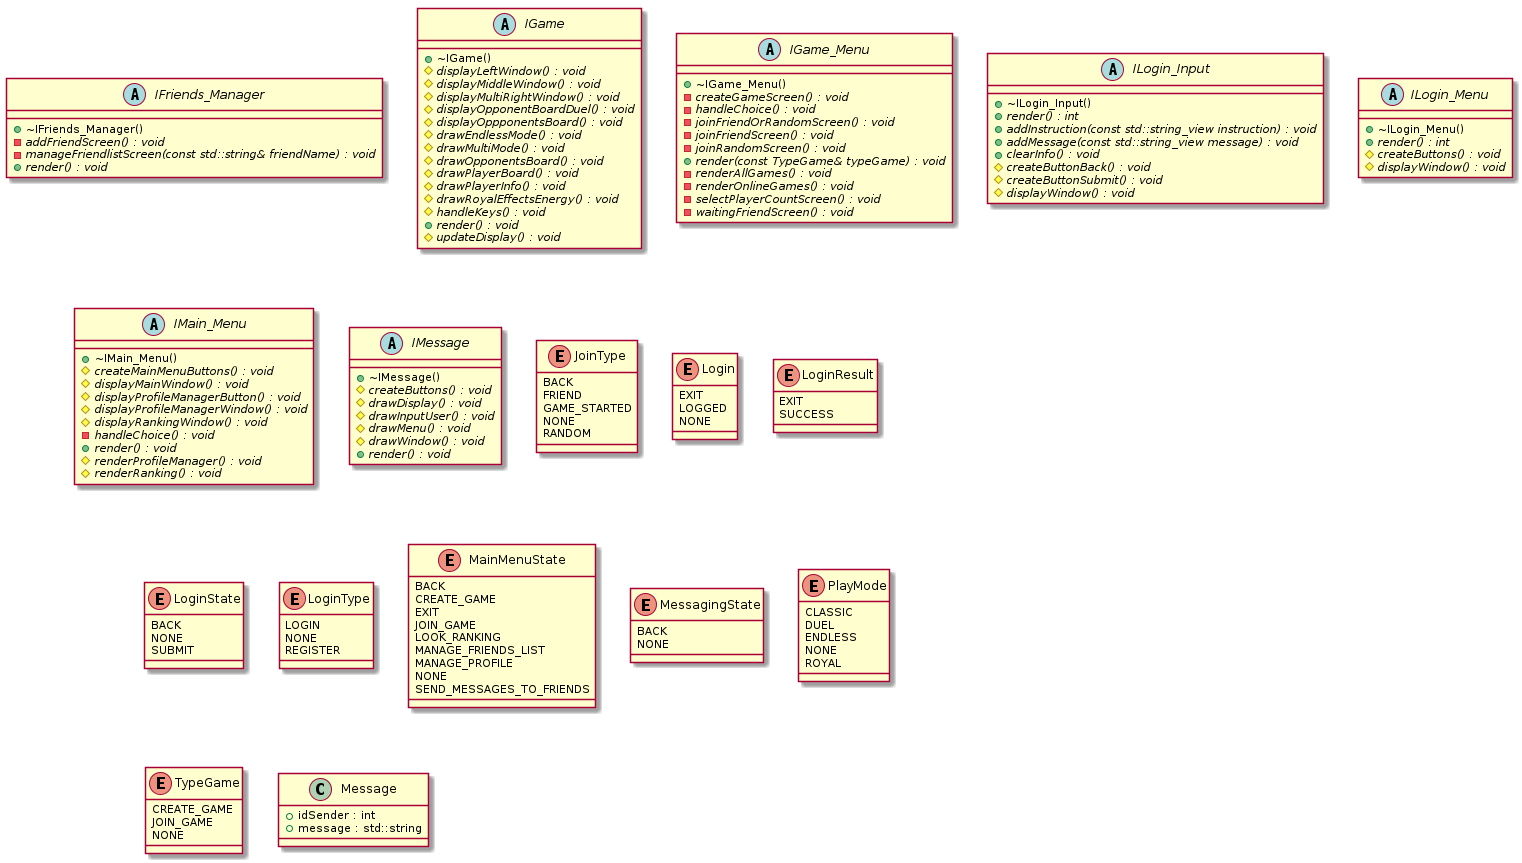
\includegraphics[width=1\textwidth]{../../res/uml/class/InterfaceClass.png}
%\end{frame}

\subsection{Implémentation avec ftxui}
\begin{frame}
\frametitle{Implémentation avec ftxui}

\includegraphics[width=1\textwidth]{../../res/uml/class/InterfaceFTXUIClass.png}
\end{frame}

\subsection{Implémentation générale}
\begin{frame}
\frametitle{Implémentation générale du Client}

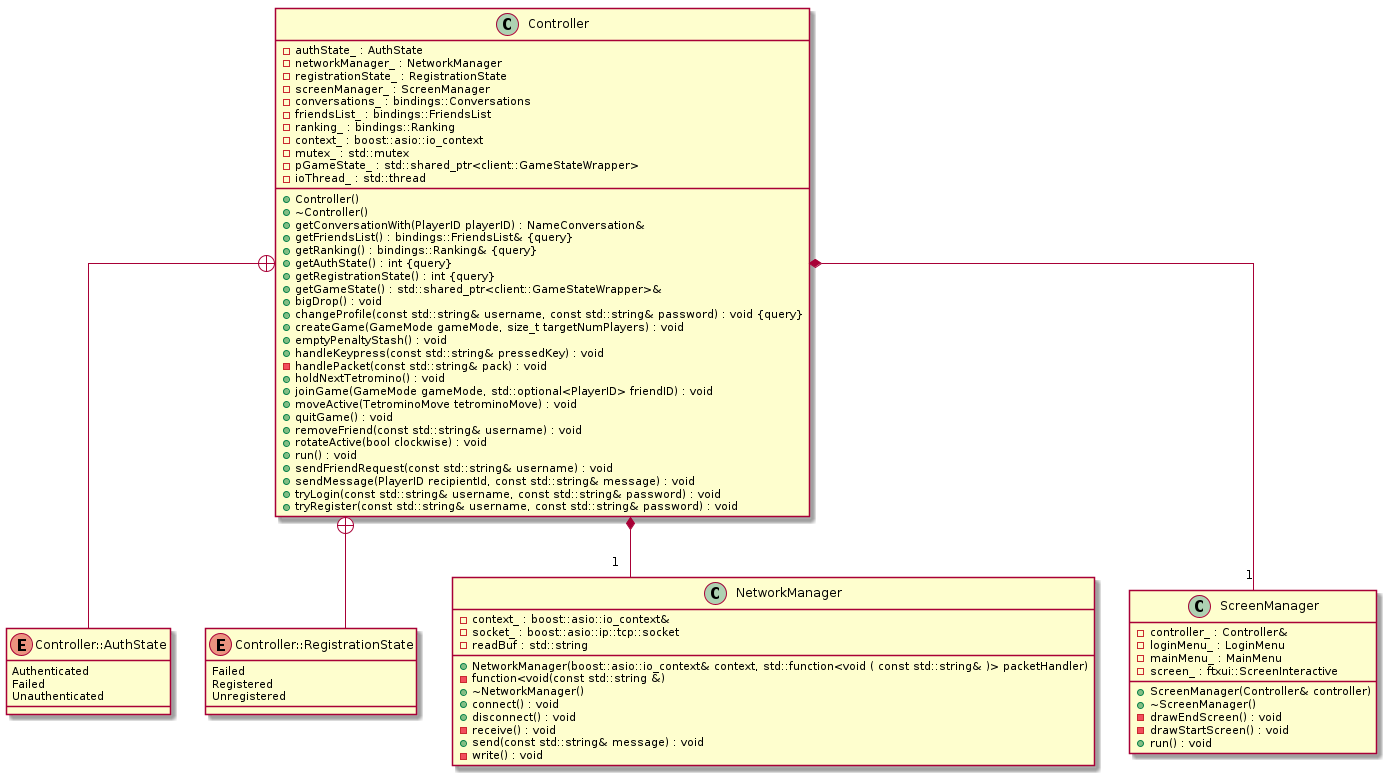
\includegraphics[width=1\textwidth]{../../res/uml/class/ClientStructureClass.png}
\end{frame}

\subsection{Fonctionnement}


\subsubsection{Game}
\begin{frame}
\frametitle{Fonctionnement du jeu côté client}

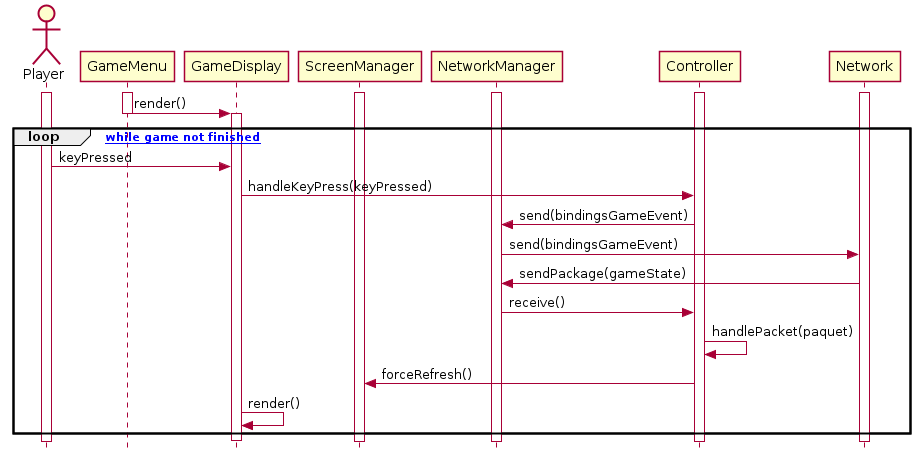
\includegraphics[width=1\textwidth]{../../res/uml/sequence/GameClientSequence.png}
\end{frame}

\subsubsection{MatchMaking}
\begin{frame}
\frametitle{Fonctionnement du Matchmaking côté client}

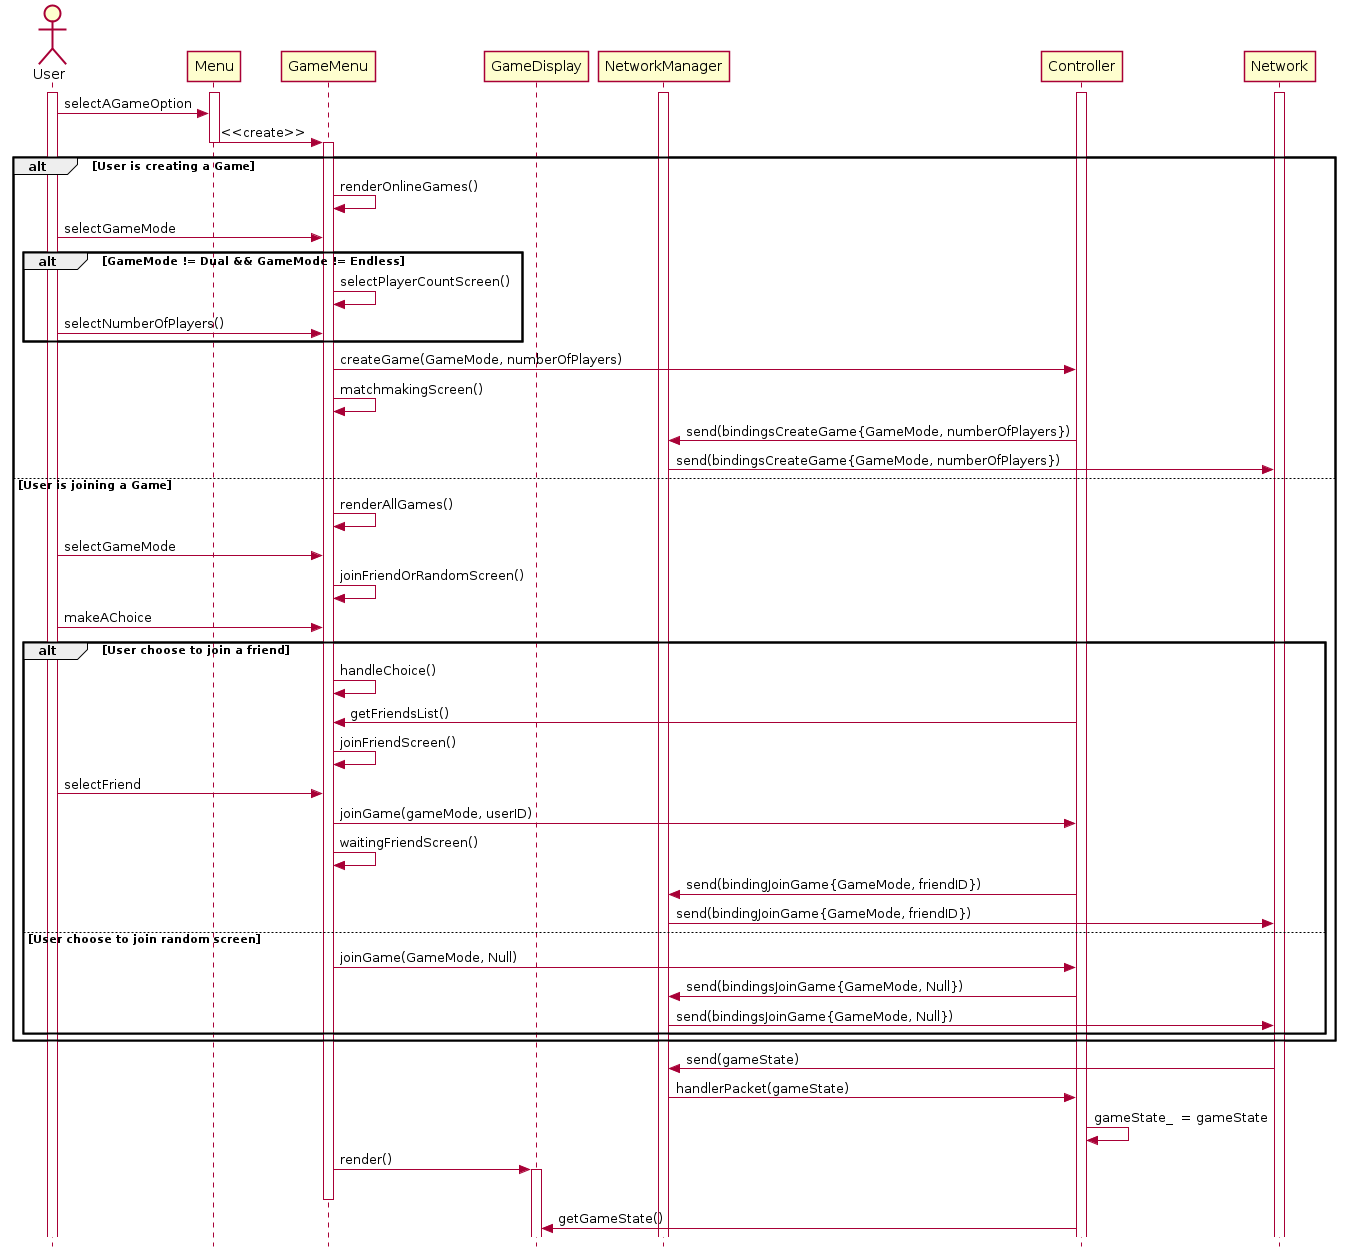
\includegraphics[width=1\textwidth]{../../res/uml/sequence/MatchMakingClientSequence.png}
\end{frame}

\subsubsection{Inscription}
\begin{frame}
\frametitle{Fonctionnement de l'inscription}

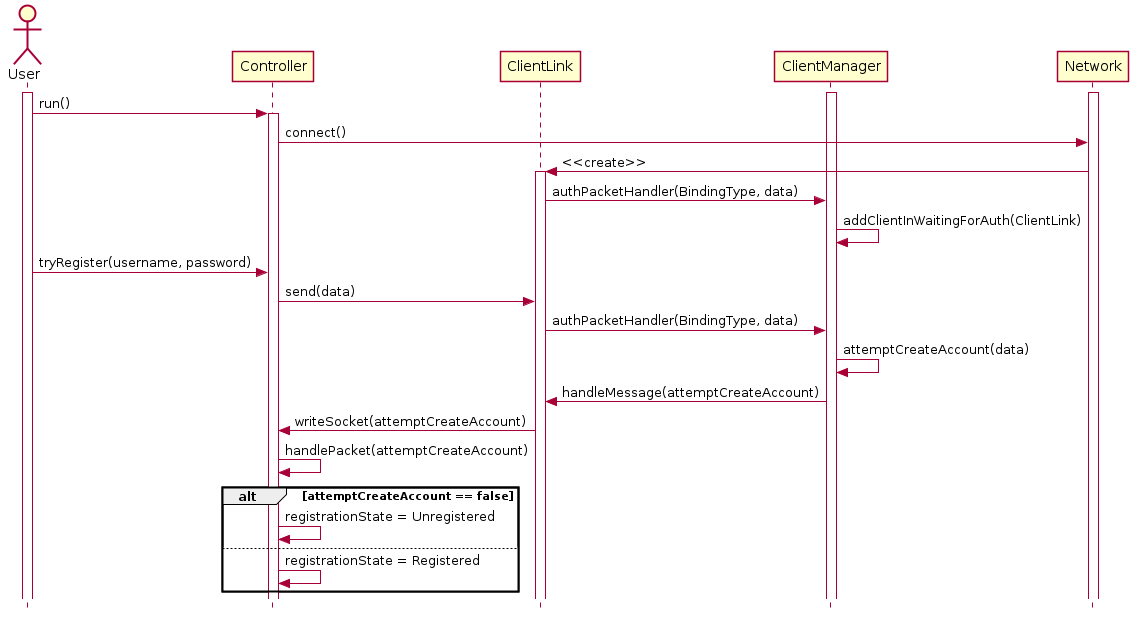
\includegraphics[width=1\textwidth]{../../res/uml/sequence/InscriptionSequence.png}
\end{frame}

\subsubsection{Connexion}
\begin{frame}
\frametitle{Fonctionnement de l'authentification du client}

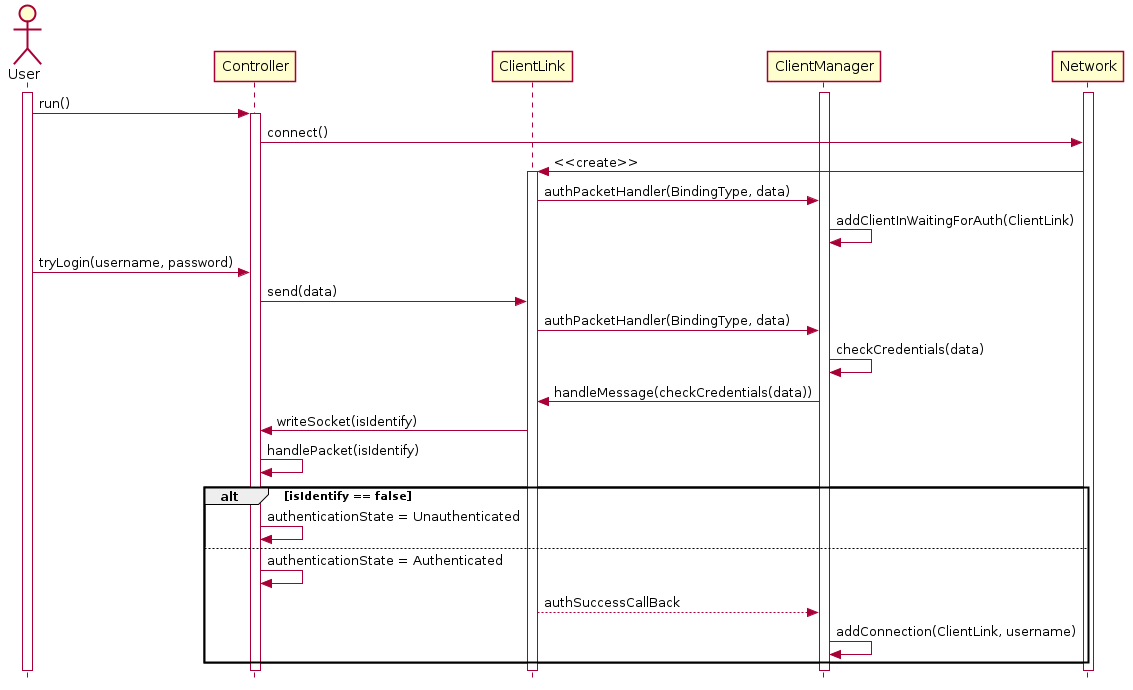
\includegraphics[width=1\textwidth]{../../res/uml/sequence/ConnexionSequence.png}
\end{frame}

\section{Pour la phase 3}
\begin{frame}
\frametitle{Pour la phase 3}

\begin{enumerate}
	\item GUI
	\item mode royal 
	\item mode spectateur
	\item rejoindre un ami dans une partie
\end{enumerate}
\end{frame}

\end{document}